\section{XMList\-Base\-Class  Class Reference}
\label{classXMListBaseClass}\index{XMListBaseClass@{XMList\-Base\-Class}}
{\tt \#include $<$XMList.h$>$}

Inheritance diagram for XMList\-Base\-Class::\begin{figure}[H]
\begin{center}
\leavevmode
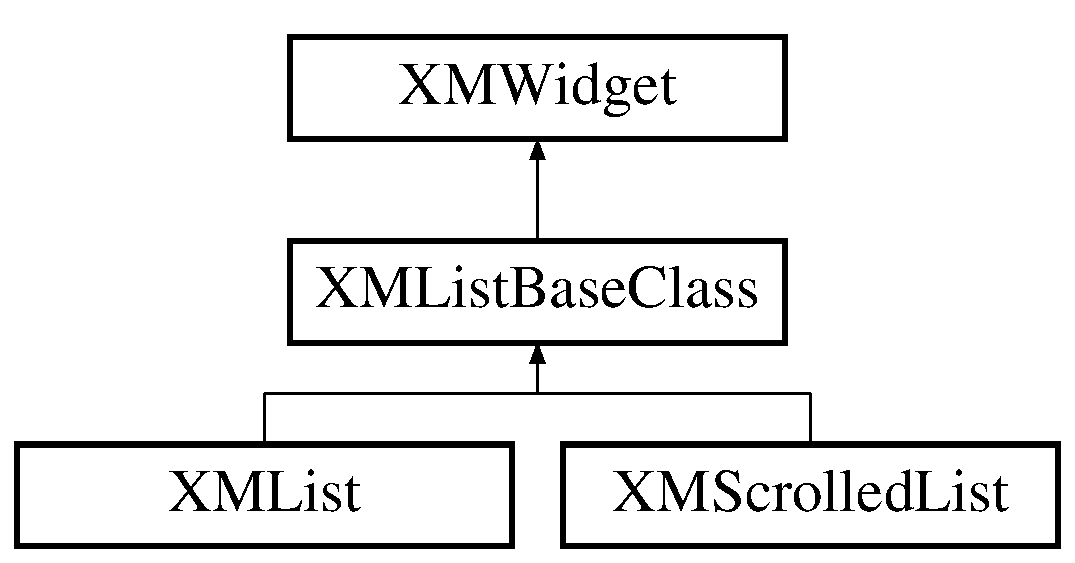
\includegraphics[height=3cm]{classXMListBaseClass}
\end{center}
\end{figure}
\subsection*{Public Methods}
\begin{CompactItemize}
\item 
{\bf XMList\-Base\-Class} (char $\ast$n, Widget\-Class cl, {\bf XMWidget} \&parent, Arg\-List l=NULL, Cardinal num\_\-args=0)
\item 
{\bf XMList\-Base\-Class} (char $\ast$n, Widget\-Class cl, Widget parent, Arg\-List l=NULL, Cardinal num\_\-args=0)
\item 
{\bf XMList\-Base\-Class} (char $\ast$n)
\item 
{\bf XMList\-Base\-Class} (Widget w)
\item 
void {\bf Auto\-Select} (Boolean enable=True)
\item 
void {\bf Set\-Double\-Click\-Time} (int ms=100)
\item 
void {\bf Set\-Rows} (int rows)
\item 
void {\bf Set\-Scroll\-Policy} (int policy=Xm\-AS\_\-NEEDED)
\item 
void {\bf Set\-Selection\-Policy} (int policy=Xm\-SINGLE\_\-SELECT)
\item 
int {\bf Get\-List\-Count} ()
\item 
Xm\-String\-Table {\bf Get\-List\-Values} ()
\item 
int {\bf Get\-Selected\-List\-Count} ()
\item 
Xm\-String\-Table {\bf Get\-Selected\-Items} ()
\item 
{\bf Callback\_\-data} $\ast$ {\bf Addbrowse\-Selection\-Callback} (void($\ast$callback)({\bf XMWidget} $\ast$, Xt\-Pointer, Xt\-Pointer), Xt\-Pointer user\_\-data=NULL)
\item 
{\bf Callback\_\-data} $\ast$ {\bf Add\-Default\-Action\-Callback} (void($\ast$callback)({\bf XMWidget} $\ast$, Xt\-Pointer, Xt\-Pointer), Xt\-Pointer user\_\-data=NULL)
\item 
{\bf Callback\_\-data} $\ast$ {\bf Add\-Extended\-Selection\-Callback} (void($\ast$callback)({\bf XMWidget} $\ast$, Xt\-Pointer, Xt\-Pointer), Xt\-Pointer user\_\-data=NULL)
\item 
{\bf Callback\_\-data} $\ast$ {\bf Add\-Multiple\-Selection\-Callback} (void($\ast$callback)({\bf XMWidget} $\ast$, Xt\-Pointer, Xt\-Pointer), Xt\-Pointer user\_\-data=NULL)
\item 
{\bf Callback\_\-data} $\ast$ {\bf Add\-Single\-Selection\-Callback} (void($\ast$callback)({\bf XMWidget} $\ast$, Xt\-Pointer, Xt\-Pointer), Xt\-Pointer user\_\-data=NULL)
\item 
void {\bf Add\-Item} (char $\ast$item, int position=0)
\item 
void {\bf Clear\-Items} ()
\item 
void {\bf Delete\-Item} (char $\ast$item)
\item 
void {\bf Delete\-Item} (int loc=0)
\item 
void {\bf Delete\-Items} (int loc, int count=1)
\item 
void {\bf Deselect\-All} ()
\item 
void {\bf Deselect\-Item} (char $\ast$item)
\item 
void {\bf Deselect\-Item} (int pos=0)
\item 
void {\bf Set\-Bottom\-Item} (int position=0)
\item 
void {\bf Select\-Item} (int pos=0)
\end{CompactItemize}


\subsection{Constructor \& Destructor Documentation}
\index{XMListBaseClass@{XMList\-Base\-Class}!XMListBaseClass@{XMListBaseClass}}
\index{XMListBaseClass@{XMListBaseClass}!XMListBaseClass@{XMList\-Base\-Class}}
\subsubsection{\setlength{\rightskip}{0pt plus 5cm}XMList\-Base\-Class::XMList\-Base\-Class (char $\ast$ {\em n}, Widget\-Class {\em cl}, {\bf XMWidget} \& {\em parent}, Arg\-List {\em l} = NULL, Cardinal {\em num\_\-args} = 0)\hspace{0.3cm}{\tt  [inline]}}\label{classXMListBaseClass_a0}




Definition at line 311 of file XMList.h.\index{XMListBaseClass@{XMList\-Base\-Class}!XMListBaseClass@{XMListBaseClass}}
\index{XMListBaseClass@{XMListBaseClass}!XMListBaseClass@{XMList\-Base\-Class}}
\subsubsection{\setlength{\rightskip}{0pt plus 5cm}XMList\-Base\-Class::XMList\-Base\-Class (char $\ast$ {\em n}, Widget\-Class {\em cl}, Widget {\em parent}, Arg\-List {\em l} = NULL, Cardinal {\em num\_\-args} = 0)\hspace{0.3cm}{\tt  [inline]}}\label{classXMListBaseClass_a1}




Definition at line 314 of file XMList.h.\index{XMListBaseClass@{XMList\-Base\-Class}!XMListBaseClass@{XMListBaseClass}}
\index{XMListBaseClass@{XMListBaseClass}!XMListBaseClass@{XMList\-Base\-Class}}
\subsubsection{\setlength{\rightskip}{0pt plus 5cm}XMList\-Base\-Class::XMList\-Base\-Class (char $\ast$ {\em n})\hspace{0.3cm}{\tt  [inline]}}\label{classXMListBaseClass_a2}




Definition at line 318 of file XMList.h.\index{XMListBaseClass@{XMList\-Base\-Class}!XMListBaseClass@{XMListBaseClass}}
\index{XMListBaseClass@{XMListBaseClass}!XMListBaseClass@{XMList\-Base\-Class}}
\subsubsection{\setlength{\rightskip}{0pt plus 5cm}XMList\-Base\-Class::XMList\-Base\-Class (Widget {\em w})\hspace{0.3cm}{\tt  [inline]}}\label{classXMListBaseClass_a3}




Definition at line 319 of file XMList.h.

\subsection{Member Function Documentation}
\index{XMListBaseClass@{XMList\-Base\-Class}!AddbrowseSelectionCallback@{AddbrowseSelectionCallback}}
\index{AddbrowseSelectionCallback@{AddbrowseSelectionCallback}!XMListBaseClass@{XMList\-Base\-Class}}
\subsubsection{\setlength{\rightskip}{0pt plus 5cm}{\bf Callback\_\-data}$\ast$ XMList\-Base\-Class::Addbrowse\-Selection\-Callback (void($\ast$ {\em callback})({\bf XMWidget} $\ast$, Xt\-Pointer, Xt\-Pointer), Xt\-Pointer {\em user\_\-data} = NULL)\hspace{0.3cm}{\tt  [inline]}}\label{classXMListBaseClass_a13}




Definition at line 364 of file XMList.h.

References XMWidget::Add\-Callback().\index{XMListBaseClass@{XMList\-Base\-Class}!AddDefaultActionCallback@{AddDefaultActionCallback}}
\index{AddDefaultActionCallback@{AddDefaultActionCallback}!XMListBaseClass@{XMList\-Base\-Class}}
\subsubsection{\setlength{\rightskip}{0pt plus 5cm}{\bf Callback\_\-data}$\ast$ XMList\-Base\-Class::Add\-Default\-Action\-Callback (void($\ast$ {\em callback})({\bf XMWidget} $\ast$, Xt\-Pointer, Xt\-Pointer), Xt\-Pointer {\em user\_\-data} = NULL)\hspace{0.3cm}{\tt  [inline]}}\label{classXMListBaseClass_a14}




Definition at line 370 of file XMList.h.

References XMWidget::Add\-Callback().\index{XMListBaseClass@{XMList\-Base\-Class}!AddExtendedSelectionCallback@{AddExtendedSelectionCallback}}
\index{AddExtendedSelectionCallback@{AddExtendedSelectionCallback}!XMListBaseClass@{XMList\-Base\-Class}}
\subsubsection{\setlength{\rightskip}{0pt plus 5cm}{\bf Callback\_\-data}$\ast$ XMList\-Base\-Class::Add\-Extended\-Selection\-Callback (void($\ast$ {\em callback})({\bf XMWidget} $\ast$, Xt\-Pointer, Xt\-Pointer), Xt\-Pointer {\em user\_\-data} = NULL)\hspace{0.3cm}{\tt  [inline]}}\label{classXMListBaseClass_a15}




Definition at line 377 of file XMList.h.

References XMWidget::Add\-Callback().\index{XMListBaseClass@{XMList\-Base\-Class}!AddItem@{AddItem}}
\index{AddItem@{AddItem}!XMListBaseClass@{XMList\-Base\-Class}}
\subsubsection{\setlength{\rightskip}{0pt plus 5cm}void XMList\-Base\-Class::Add\-Item (char $\ast$ {\em item}, int {\em position} = 0)\hspace{0.3cm}{\tt  [inline]}}\label{classXMListBaseClass_a18}




Definition at line 401 of file XMList.h.

References XMWidget::id.\index{XMListBaseClass@{XMList\-Base\-Class}!AddMultipleSelectionCallback@{AddMultipleSelectionCallback}}
\index{AddMultipleSelectionCallback@{AddMultipleSelectionCallback}!XMListBaseClass@{XMList\-Base\-Class}}
\subsubsection{\setlength{\rightskip}{0pt plus 5cm}{\bf Callback\_\-data}$\ast$ XMList\-Base\-Class::Add\-Multiple\-Selection\-Callback (void($\ast$ {\em callback})({\bf XMWidget} $\ast$, Xt\-Pointer, Xt\-Pointer), Xt\-Pointer {\em user\_\-data} = NULL)\hspace{0.3cm}{\tt  [inline]}}\label{classXMListBaseClass_a16}




Definition at line 384 of file XMList.h.

References XMWidget::Add\-Callback().\index{XMListBaseClass@{XMList\-Base\-Class}!AddSingleSelectionCallback@{AddSingleSelectionCallback}}
\index{AddSingleSelectionCallback@{AddSingleSelectionCallback}!XMListBaseClass@{XMList\-Base\-Class}}
\subsubsection{\setlength{\rightskip}{0pt plus 5cm}{\bf Callback\_\-data}$\ast$ XMList\-Base\-Class::Add\-Single\-Selection\-Callback (void($\ast$ {\em callback})({\bf XMWidget} $\ast$, Xt\-Pointer, Xt\-Pointer), Xt\-Pointer {\em user\_\-data} = NULL)\hspace{0.3cm}{\tt  [inline]}}\label{classXMListBaseClass_a17}




Definition at line 391 of file XMList.h.

References XMWidget::Add\-Callback().\index{XMListBaseClass@{XMList\-Base\-Class}!AutoSelect@{AutoSelect}}
\index{AutoSelect@{AutoSelect}!XMListBaseClass@{XMList\-Base\-Class}}
\subsubsection{\setlength{\rightskip}{0pt plus 5cm}void XMList\-Base\-Class::Auto\-Select (Boolean {\em enable} = True)\hspace{0.3cm}{\tt  [inline]}}\label{classXMListBaseClass_a4}




Definition at line 323 of file XMList.h.

References XMWidget::Set\-Attribute().\index{XMListBaseClass@{XMList\-Base\-Class}!ClearItems@{ClearItems}}
\index{ClearItems@{ClearItems}!XMListBaseClass@{XMList\-Base\-Class}}
\subsubsection{\setlength{\rightskip}{0pt plus 5cm}void XMList\-Base\-Class::Clear\-Items ()\hspace{0.3cm}{\tt  [inline]}}\label{classXMListBaseClass_a19}




Definition at line 406 of file XMList.h.

References XMWidget::id.\index{XMListBaseClass@{XMList\-Base\-Class}!DeleteItem@{DeleteItem}}
\index{DeleteItem@{DeleteItem}!XMListBaseClass@{XMList\-Base\-Class}}
\subsubsection{\setlength{\rightskip}{0pt plus 5cm}void XMList\-Base\-Class::Delete\-Item (int {\em loc} = 0)\hspace{0.3cm}{\tt  [inline]}}\label{classXMListBaseClass_a21}




Definition at line 412 of file XMList.h.

References XMWidget::id.\index{XMListBaseClass@{XMList\-Base\-Class}!DeleteItem@{DeleteItem}}
\index{DeleteItem@{DeleteItem}!XMListBaseClass@{XMList\-Base\-Class}}
\subsubsection{\setlength{\rightskip}{0pt plus 5cm}void XMList\-Base\-Class::Delete\-Item (char $\ast$ {\em item})\hspace{0.3cm}{\tt  [inline]}}\label{classXMListBaseClass_a20}




Definition at line 407 of file XMList.h.

References XMWidget::id.\index{XMListBaseClass@{XMList\-Base\-Class}!DeleteItems@{DeleteItems}}
\index{DeleteItems@{DeleteItems}!XMListBaseClass@{XMList\-Base\-Class}}
\subsubsection{\setlength{\rightskip}{0pt plus 5cm}void XMList\-Base\-Class::Delete\-Items (int {\em loc}, int {\em count} = 1)\hspace{0.3cm}{\tt  [inline]}}\label{classXMListBaseClass_a22}




Definition at line 415 of file XMList.h.

References XMWidget::id.\index{XMListBaseClass@{XMList\-Base\-Class}!DeselectAll@{DeselectAll}}
\index{DeselectAll@{DeselectAll}!XMListBaseClass@{XMList\-Base\-Class}}
\subsubsection{\setlength{\rightskip}{0pt plus 5cm}void XMList\-Base\-Class::Deselect\-All ()\hspace{0.3cm}{\tt  [inline]}}\label{classXMListBaseClass_a23}




Definition at line 418 of file XMList.h.

References XMWidget::id.\index{XMListBaseClass@{XMList\-Base\-Class}!DeselectItem@{DeselectItem}}
\index{DeselectItem@{DeselectItem}!XMListBaseClass@{XMList\-Base\-Class}}
\subsubsection{\setlength{\rightskip}{0pt plus 5cm}void XMList\-Base\-Class::Deselect\-Item (int {\em pos} = 0)\hspace{0.3cm}{\tt  [inline]}}\label{classXMListBaseClass_a25}




Definition at line 427 of file XMList.h.

References XMWidget::id.\index{XMListBaseClass@{XMList\-Base\-Class}!DeselectItem@{DeselectItem}}
\index{DeselectItem@{DeselectItem}!XMListBaseClass@{XMList\-Base\-Class}}
\subsubsection{\setlength{\rightskip}{0pt plus 5cm}void XMList\-Base\-Class::Deselect\-Item (char $\ast$ {\em item})\hspace{0.3cm}{\tt  [inline]}}\label{classXMListBaseClass_a24}




Definition at line 421 of file XMList.h.

References XMWidget::id.\index{XMListBaseClass@{XMList\-Base\-Class}!GetListCount@{GetListCount}}
\index{GetListCount@{GetListCount}!XMListBaseClass@{XMList\-Base\-Class}}
\subsubsection{\setlength{\rightskip}{0pt plus 5cm}int XMList\-Base\-Class::Get\-List\-Count ()\hspace{0.3cm}{\tt  [inline]}}\label{classXMListBaseClass_a9}




Definition at line 340 of file XMList.h.

References XMWidget::Get\-Attribute().\index{XMListBaseClass@{XMList\-Base\-Class}!GetListValues@{GetListValues}}
\index{GetListValues@{GetListValues}!XMListBaseClass@{XMList\-Base\-Class}}
\subsubsection{\setlength{\rightskip}{0pt plus 5cm}Xm\-String\-Table XMList\-Base\-Class::Get\-List\-Values ()\hspace{0.3cm}{\tt  [inline]}}\label{classXMListBaseClass_a10}




Definition at line 345 of file XMList.h.

References XMWidget::Get\-Attribute().\index{XMListBaseClass@{XMList\-Base\-Class}!GetSelectedItems@{GetSelectedItems}}
\index{GetSelectedItems@{GetSelectedItems}!XMListBaseClass@{XMList\-Base\-Class}}
\subsubsection{\setlength{\rightskip}{0pt plus 5cm}Xm\-String\-Table XMList\-Base\-Class::Get\-Selected\-Items ()\hspace{0.3cm}{\tt  [inline]}}\label{classXMListBaseClass_a12}




Definition at line 357 of file XMList.h.

References XMWidget::Get\-Attribute().\index{XMListBaseClass@{XMList\-Base\-Class}!GetSelectedListCount@{GetSelectedListCount}}
\index{GetSelectedListCount@{GetSelectedListCount}!XMListBaseClass@{XMList\-Base\-Class}}
\subsubsection{\setlength{\rightskip}{0pt plus 5cm}int XMList\-Base\-Class::Get\-Selected\-List\-Count ()\hspace{0.3cm}{\tt  [inline]}}\label{classXMListBaseClass_a11}




Definition at line 351 of file XMList.h.

References XMWidget::Get\-Attribute().\index{XMListBaseClass@{XMList\-Base\-Class}!SelectItem@{SelectItem}}
\index{SelectItem@{SelectItem}!XMListBaseClass@{XMList\-Base\-Class}}
\subsubsection{\setlength{\rightskip}{0pt plus 5cm}void XMList\-Base\-Class::Select\-Item (int {\em pos} = 0)\hspace{0.3cm}{\tt  [inline]}}\label{classXMListBaseClass_a27}




Definition at line 434 of file XMList.h.

References XMWidget::id.\index{XMListBaseClass@{XMList\-Base\-Class}!SetBottomItem@{SetBottomItem}}
\index{SetBottomItem@{SetBottomItem}!XMListBaseClass@{XMList\-Base\-Class}}
\subsubsection{\setlength{\rightskip}{0pt plus 5cm}void XMList\-Base\-Class::Set\-Bottom\-Item (int {\em position} = 0)\hspace{0.3cm}{\tt  [inline]}}\label{classXMListBaseClass_a26}




Definition at line 430 of file XMList.h.

References XMWidget::id.\index{XMListBaseClass@{XMList\-Base\-Class}!SetDoubleClickTime@{SetDoubleClickTime}}
\index{SetDoubleClickTime@{SetDoubleClickTime}!XMListBaseClass@{XMList\-Base\-Class}}
\subsubsection{\setlength{\rightskip}{0pt plus 5cm}void XMList\-Base\-Class::Set\-Double\-Click\-Time (int {\em ms} = 100)\hspace{0.3cm}{\tt  [inline]}}\label{classXMListBaseClass_a5}




Definition at line 326 of file XMList.h.

References XMWidget::Set\-Attribute().\index{XMListBaseClass@{XMList\-Base\-Class}!SetRows@{SetRows}}
\index{SetRows@{SetRows}!XMListBaseClass@{XMList\-Base\-Class}}
\subsubsection{\setlength{\rightskip}{0pt plus 5cm}void XMList\-Base\-Class::Set\-Rows (int {\em rows})\hspace{0.3cm}{\tt  [inline]}}\label{classXMListBaseClass_a6}




Definition at line 330 of file XMList.h.

References XMWidget::Set\-Attribute().

Referenced by XMList::XMList(), and XMScrolled\-List::XMScrolled\-List().\index{XMListBaseClass@{XMList\-Base\-Class}!SetScrollPolicy@{SetScrollPolicy}}
\index{SetScrollPolicy@{SetScrollPolicy}!XMListBaseClass@{XMList\-Base\-Class}}
\subsubsection{\setlength{\rightskip}{0pt plus 5cm}void XMList\-Base\-Class::Set\-Scroll\-Policy (int {\em policy} = Xm\-AS\_\-NEEDED)\hspace{0.3cm}{\tt  [inline]}}\label{classXMListBaseClass_a7}




Definition at line 333 of file XMList.h.

References XMWidget::Set\-Attribute().\index{XMListBaseClass@{XMList\-Base\-Class}!SetSelectionPolicy@{SetSelectionPolicy}}
\index{SetSelectionPolicy@{SetSelectionPolicy}!XMListBaseClass@{XMList\-Base\-Class}}
\subsubsection{\setlength{\rightskip}{0pt plus 5cm}void XMList\-Base\-Class::Set\-Selection\-Policy (int {\em policy} = Xm\-SINGLE\_\-SELECT)\hspace{0.3cm}{\tt  [inline]}}\label{classXMListBaseClass_a8}




Definition at line 336 of file XMList.h.

References XMWidget::Set\-Attribute().

The documentation for this class was generated from the following file:\begin{CompactItemize}
\item 
{\bf XMList.h}\end{CompactItemize}
